\title{Project 2}
\author{
        Jerry Duncan
}
\date{\today}

\documentclass[12pt]{article}

\usepackage{amsmath}
\usepackage{graphicx}
\usepackage{pythonhighlight}


\begin{document}
\maketitle

\section{Introduction}

For this project, we are taking a look at a simple Reinforcement Learning problem where there exists a small, $d$x$d$ grid and there exists a robot and bomb somewhere on this grid. Our goal is to teach the robot how to get the bomb off the grid as quickly as possible. We will apply two different methods to this problem, Q-Learning and First-Visit Monte Carlo, to see which performs better at a) generally solving the problem and b) which does so in the fastest manner. First we will form the problem as an MDP, where the state consists of the robot and bomb's position. Then we will apply those two methods using two different reward structures and 2 different behavior policies in the case of Q-Learning, to see how well they solve the problem. And lastly, we will compare the time it takes for them to converge to their solutions.

\paragraph{Important Note} I set up my problem so that if we don't push the bomb out by step 1,000, we lose the problem. This means that we will still use the episode to learn for the MC Learning because this greatly simplified the programming for the problem. It still converges and works, but it does mean that some of the Q values are a lot larger than might be expected when talking about them in the Results.

\section{Markov Decision Process}

\paragraph{State space} The state space for this problem is very simple. The environment must keep track of two things and allow the robot to know of those two things: robot X, robot Y, bomb X, and bomb Y. This means the dimensionality of the state space ends up being $d^4$ and since $d = 8$ then the state space has $4096$ total states.

\paragraph{Action space} The only actions our robot can take at any state are the cardinal directions $N, E, S, W$. So our action space $A = { N, E, S, W }$ for each and every state.

\paragraph{Reward Structure} We want to test out two different reward structures, both of which are given to us. The first is to always give a -1 reward regardless of move. The other, is more complicated, but gives +10 when the robot puts the bomb in the river, +1 when the robot moves the bomb further away from the center of the grid, and -1 for any other move.

\section{Code and Data Structures}
I used a class-based structure for this project to keep all data close to its source. The environment is modeled as a class that has the following methods:
\begin{itemize}
  \item \textit{start}: Initializes a random starting state to begin an episode
  \item \textit{move}: Takes an action, given the current state, and moves the robot (and bomb if necessary), as well as returning the reward for that action
  \item \textit{reward}: Determines the reward based on a given state and action and which reward structure being used
  \item Helpers
        \begin{itemize}
          \item \textit{dist}: Calculates the distance from the center of the board to an arbitrary position
          \item \textit{next\_position}: Calculates the next position given a current position and an action
        \end{itemize}
\end{itemize}

The MCLearner and QLearner classes subclass Learner. All Learners are structured as follows:
\begin{itemize}
  \item \textit{\_\_init\_\_}: Initializes an array for Q values and for the policy
  \item \textit{learn}: Generates episodes and learns on them, depending on the type of learning (Q or MC)
  \item \textit{run}: Runs the learning function $n$ times.
  \item \textit{plot}: Takes a starting state, generates an episode, and plots it
  \item Helpers
        \begin{itemize}
          \item \textit{final\_policy}: Prepares the learned policy for use in episodes after training
          \item \textit{q\_values}: Runs an episode and prints out the Q values
        \end{itemize}
\end{itemize}

\section{Results}

All experiments are performed over 50,000 episodes.

Before we start looking at results and discussing why they make sense, let's first determine what should the optimal route given the constant or dynamic reward structure be?

Given the board from the assignment, we as humans can see the optimal path has to be 5 moves long because there is no shorter path that can get the bomb off the grid. And for the constant reward structure, the optimal path overall is the same as the optimal path for maximizing the reward. Specifically, that sequence of actions would be: East, East, North, West, and West for a total of -5 reward. However, for the dynamic reward structure, we get +1 when we move the bomb further away from the center. This means that we can potentially make up for some of our earlier -1 moves by taking some +1 moves. While it may not be obvious at first glance, I propose that the following sequence of actions would product a higher reward than the ones used for the constant reward structure: East, North, North, North, North, North. This set of actions gives us a reward of 11 versus 8 for the action set from the optimal constant reward path. This is because while the first two actions are normal steps and we receive -2, the third, fourth, and fifth action all move the box further away from the center giving us +3 and the 6th final action gives us +10 for removing it from the board for a total of 11. It also contains 6 actions, meaning it's impossible to be the optimal for the constant reward structure. I propose that since these two paths are the optimal, they should be what we expect our models to learn. Make note that the 6-move optimal path for maximizing the reward for the dynamic reward structure is not optimal for the problem itself, but this is a failing of the dynamic reward structure.

\paragraph{Part a}

\textbf{Q-Learning with a Constant Reward and a Uniform Policy}
\begin{itemize}
  \item Q((robotX: 0, robotY: 5), (bombX: 1, bombY: 4)) = [N: -7.00, E: -5.00, S: -7.00, W: -6.00]
  \item Q((robotX: 1, robotY: 5), (bombX: 1, bombY: 4)) = [N: -5.00, E: -4.00, S: -6.00, W: -6.00]
  \item Q((robotX: 2, robotY: 5), (bombX: 1, bombY: 4)) = [N: -3.00, E: -5.00, S: -5.00, W: -5.00]
  \item Q((robotX: 2, robotY: 4), (bombX: 1, bombY: 4)) = [N: -4.00, E: -4.00, S: -4.00, W: -2.00]
  \item Q((robotX: 1, robotY: 4), (bombX: 0, bombY: 4)) = [N: -3.00, E: -3.00, S: -3.00, W: -1.00]
\end{itemize}

We end up with nice, round whole numbers because our policy has forced us to take each action equally, meaning that our estimates of the Q's are more likely to be accurate.

\textbf{Q-Learning with a Constant Reward and a Greedy Policy}
\begin{itemize}
  \item Q((robotX: 0, robotY: 5), (bombX: 1, bombY: 4)) = [N: -4.90, E: -4.81, S: -4.94, W: -4.85]
  \item Q((robotX: 1, robotY: 5), (bombX: 1, bombY: 4)) = [N: -4.08, E: -4.00, S: -4.28, W: -4.18]
  \item Q((robotX: 2, robotY: 5), (bombX: 1, bombY: 4)) = [N: -3.00, E: -4.01, S: -4.54, W: -3.43]
  \item Q((robotX: 2, robotY: 4), (bombX: 1, bombY: 4)) = [N: -3.99, E: -3.96, S: -3.98, W: -2.00]
  \item Q((robotX: 1, robotY: 4), (bombX: 0, bombY: 4)) = [N: -3.00, E: -3.00, S: -3.00, W: -1.00]
\end{itemize}

While we still end up with the right path when using a greedy policy, the estimated Q values are less accurate because despite going through 50,000 episodes, the chances that we visit these specific states and don't pick the greedy action are still relatively low. If we had trained longer, these would have converged further, nevertheless they're still good enough to find the optimal solution for this reward structure.


\textbf{Monte Carlo First-Visit with a Constant Reward}
\begin{itemize}
  \item Q((robotX: 0, robotY: 5), (bombX: 1, bombY: 4)) = [N: -198.30, E: -203.12, S: -12.68, W: -183.27]
  \item Q((robotX: 0, robotY: 6), (bombX: 1, bombY: 4)) = [N: -95.39, E: -73.63, S: -10.66, W: -58.54]
  \item Q((robotX: 0, robotY: 7), (bombX: 1, bombY: 4)) = [N: -163.37, E: -8.65, S: -136.27, W: -126.16]
  \item Q((robotX: 1, robotY: 7), (bombX: 1, bombY: 4)) = [N: -257.84, E: -6.83, S: -165.50, W: -118.29]
  \item Q((robotX: 2, robotY: 7), (bombX: 1, bombY: 4)) = [N: -5.59, E: -150.20, S: -210.05, W: -212.83]
  \item Q((robotX: 2, robotY: 6), (bombX: 1, bombY: 4)) = [N: -5.01, E: -119.67, S: -182.41, W: -142.35]
  \item Q((robotX: 2, robotY: 5), (bombX: 1, bombY: 4)) = [N: -3.35, E: -102.30, S: -64.37, W: -88.88]
  \item Q((robotX: 2, robotY: 4), (bombX: 1, bombY: 4)) = [N: -33.09, E: -54.13, S: -39.45, W: -2.06]
  \item Q((robotX: 1, robotY: 4), (bombX: 0, bombY: 4)) = [N: -4.34, E: -3.61, S: -6.67, W: -1.00]
\end{itemize}

Because the episodes are so long, our initial estimates of Q can be very large. Especially because each state is so rare to occur and exploration is still somewhat rare.

\paragraph{Part b} The path taken by \textbf{Q-Learning with a Constant Reward and a Uniform Policy} is shown in Figure \ref{fig:qcu}. It makes sense that we found the optimal path because a our Q estimates have converged perfectly for this scenario and our final policy can easily find this path. The path taken by \textbf{Q-Learning with a Constant Reward and a Greedy Policy} is shown in Figure \ref{fig:qcg}. Similar to the uniform policy Q learner, this one has near-perfect Q estimates and can still easily find the path. And the path taken by \textbf{Monte Carlo First-Visit with a Constant Reward} is shown in Figure \ref{fig:mcc}. The Monte Carlo path is a bit rough and nowhere near optimal. The reason for this is likely because the first time we solved this scenario in our training, it was nonoptimal and we didn't explore enough to find better Q estimates.

\begin{figure}
  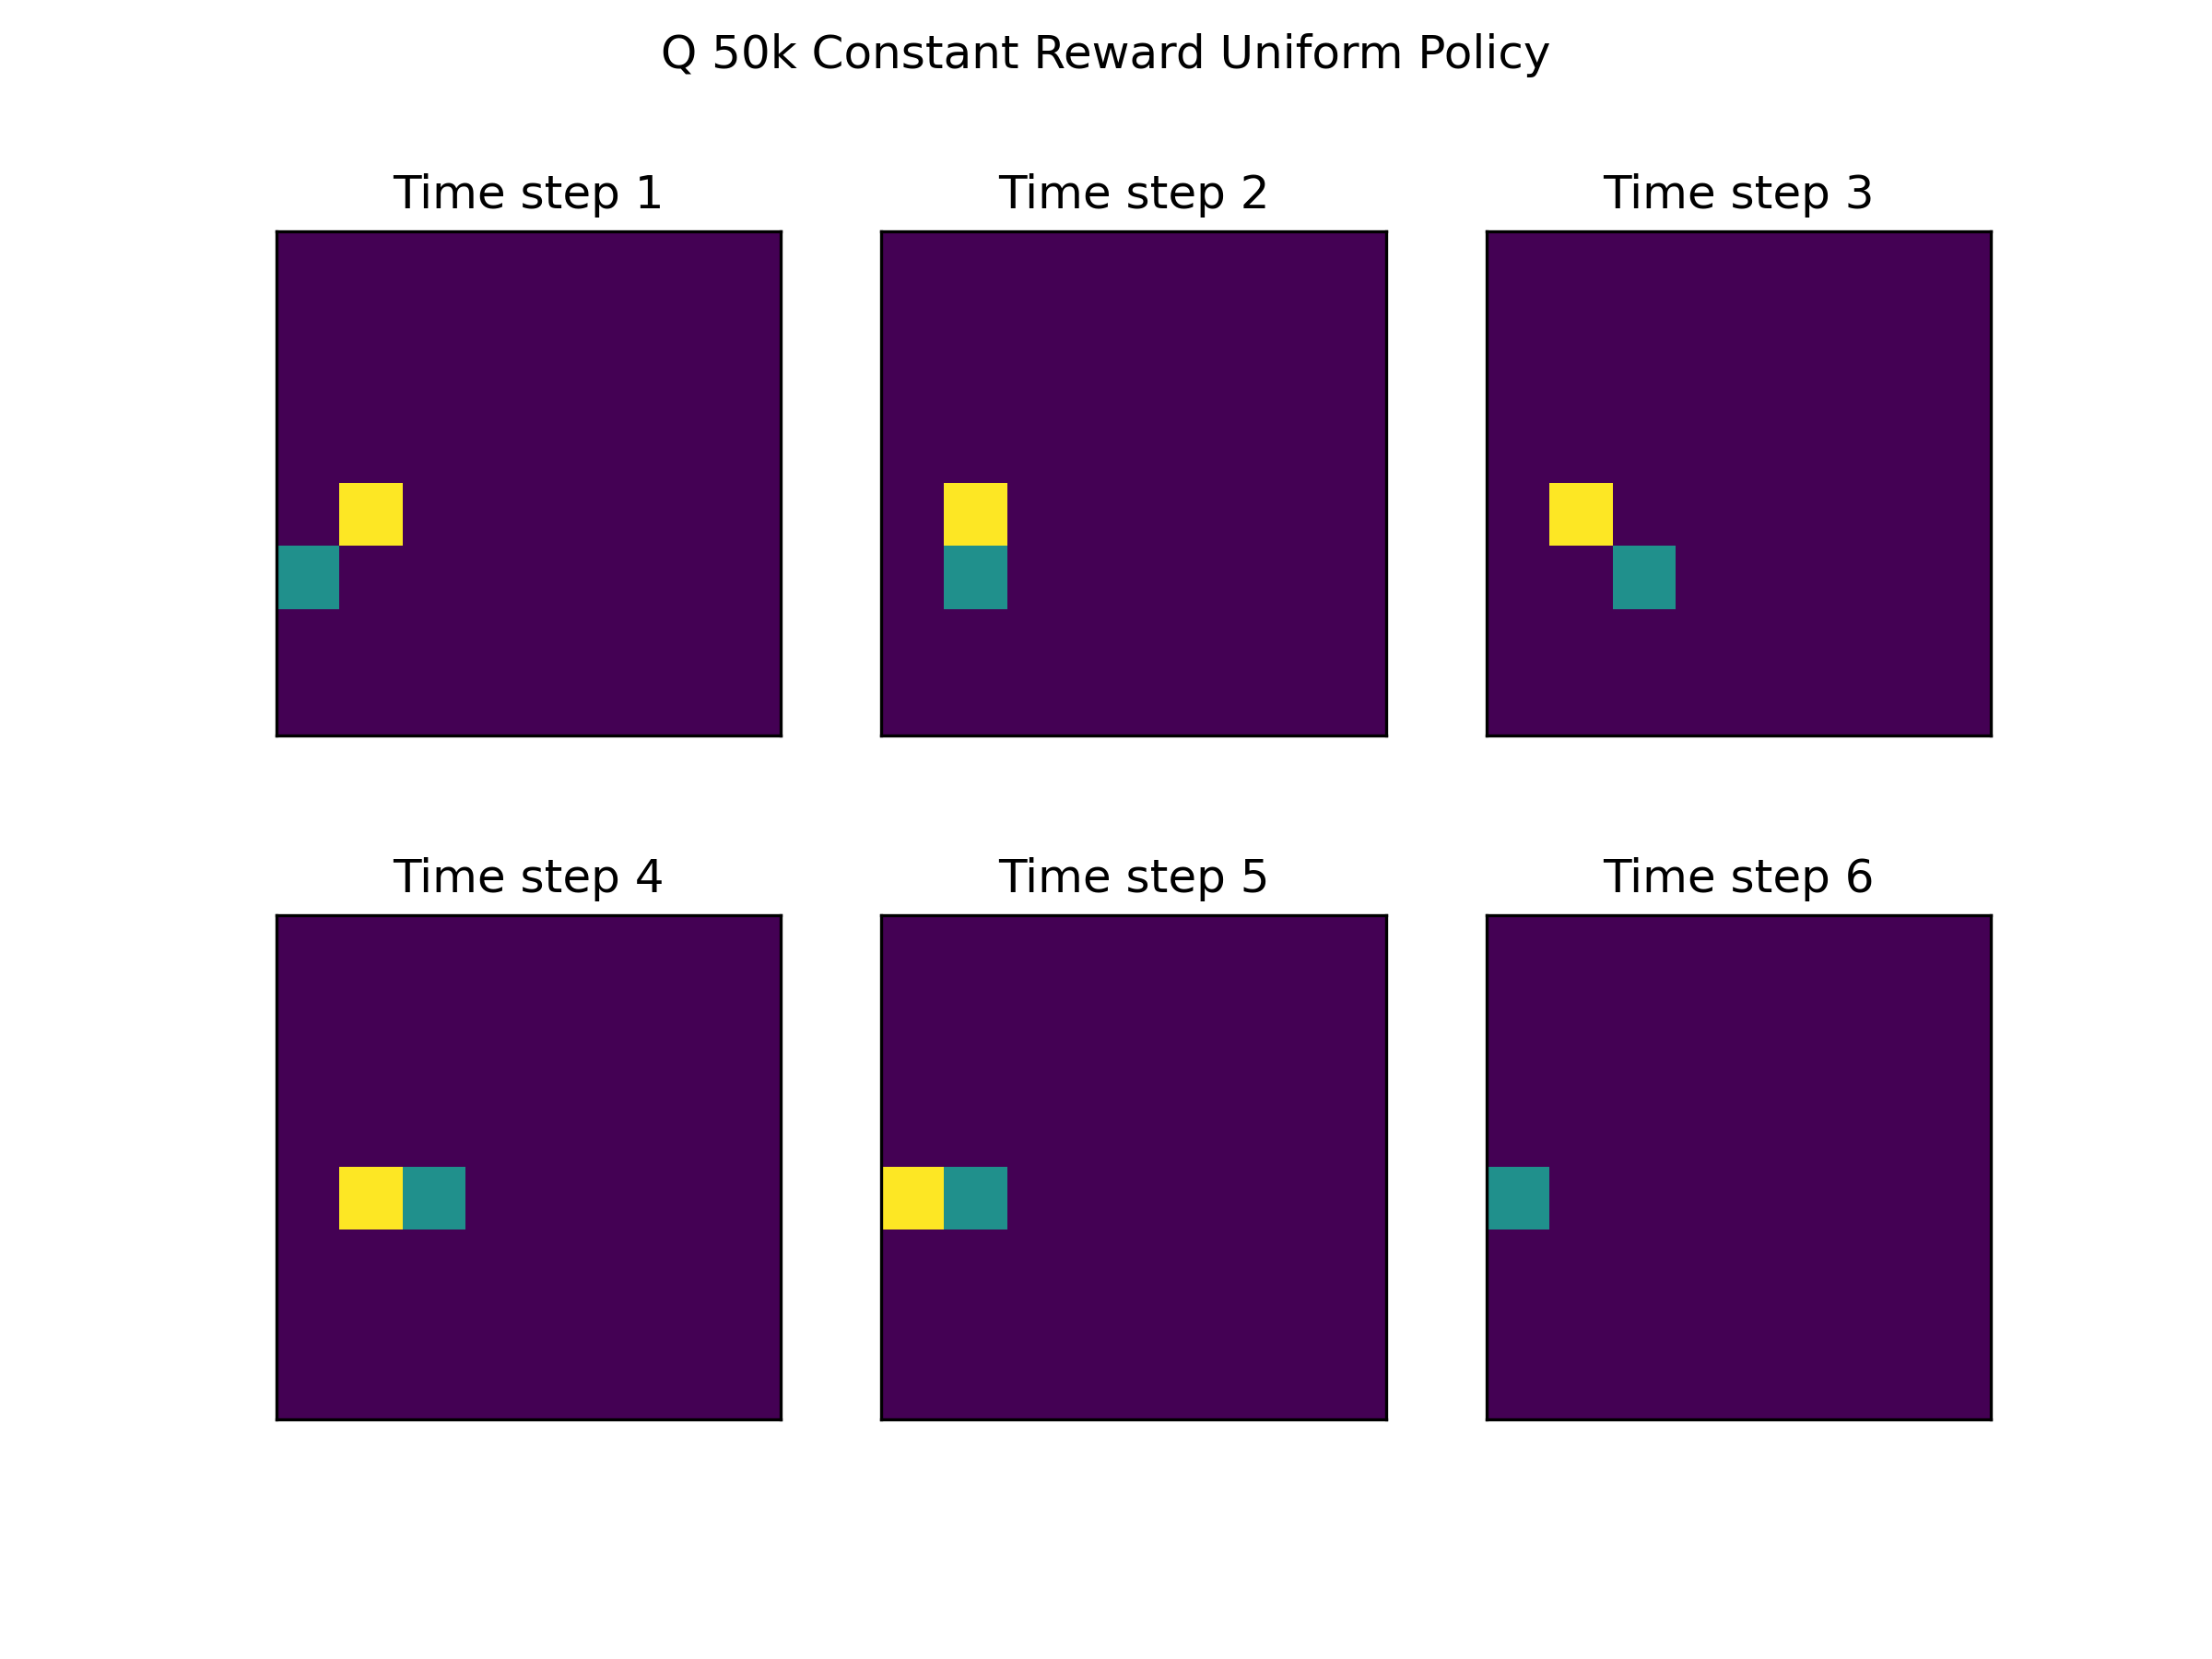
\includegraphics[width=0.95\linewidth]{Figures/q-50k-constant-reward-uniform-policy.png}
  \centering
  \label{fig:qcu}
  \caption{The path taken by the Q-Learning robot with a Constant Reward and a Uniform Policy. Blue-green is the robot. Yellow is the bomb.}
\end{figure}

\begin{figure}
  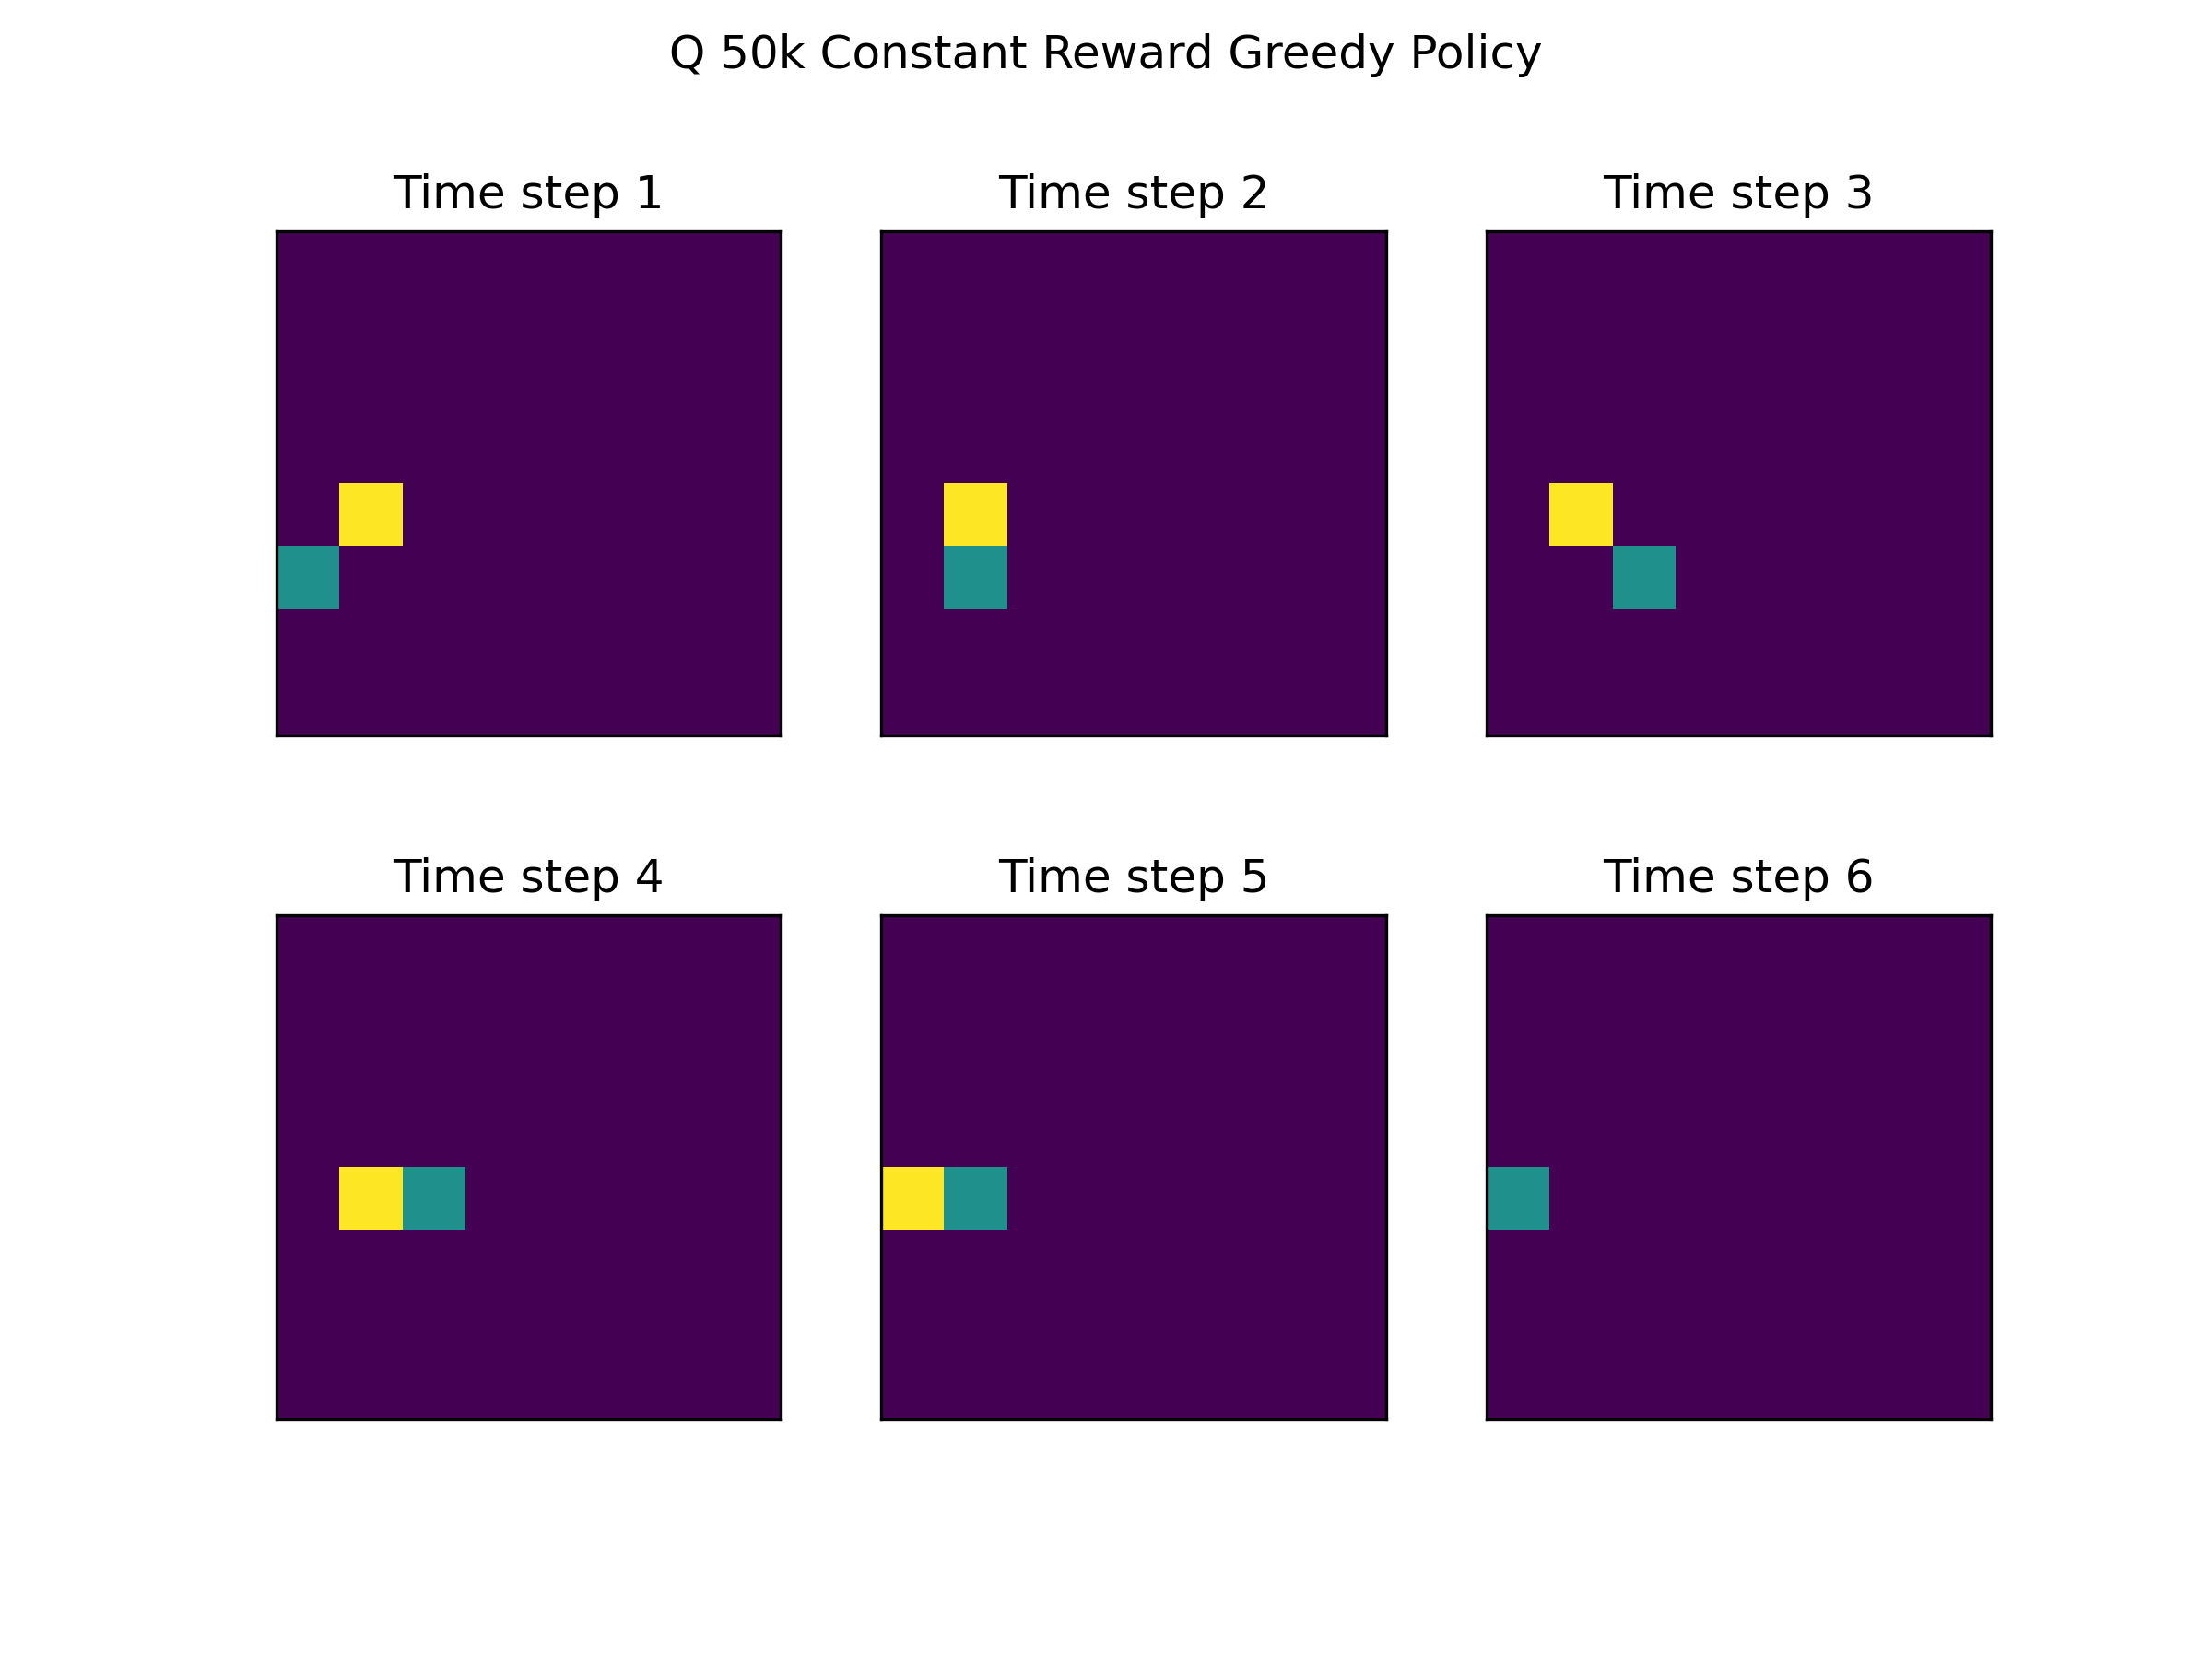
\includegraphics[width=0.95\linewidth]{Figures/q-50k-constant-reward-greedy-policy.png}
  \centering
  \label{fig:qcg}
  \caption{The path taken by the Q-Learning robot with a Constant Reward and a Greedy Policy. Blue-green is the robot. Yellow is the bomb.}
\end{figure}

\begin{figure}
  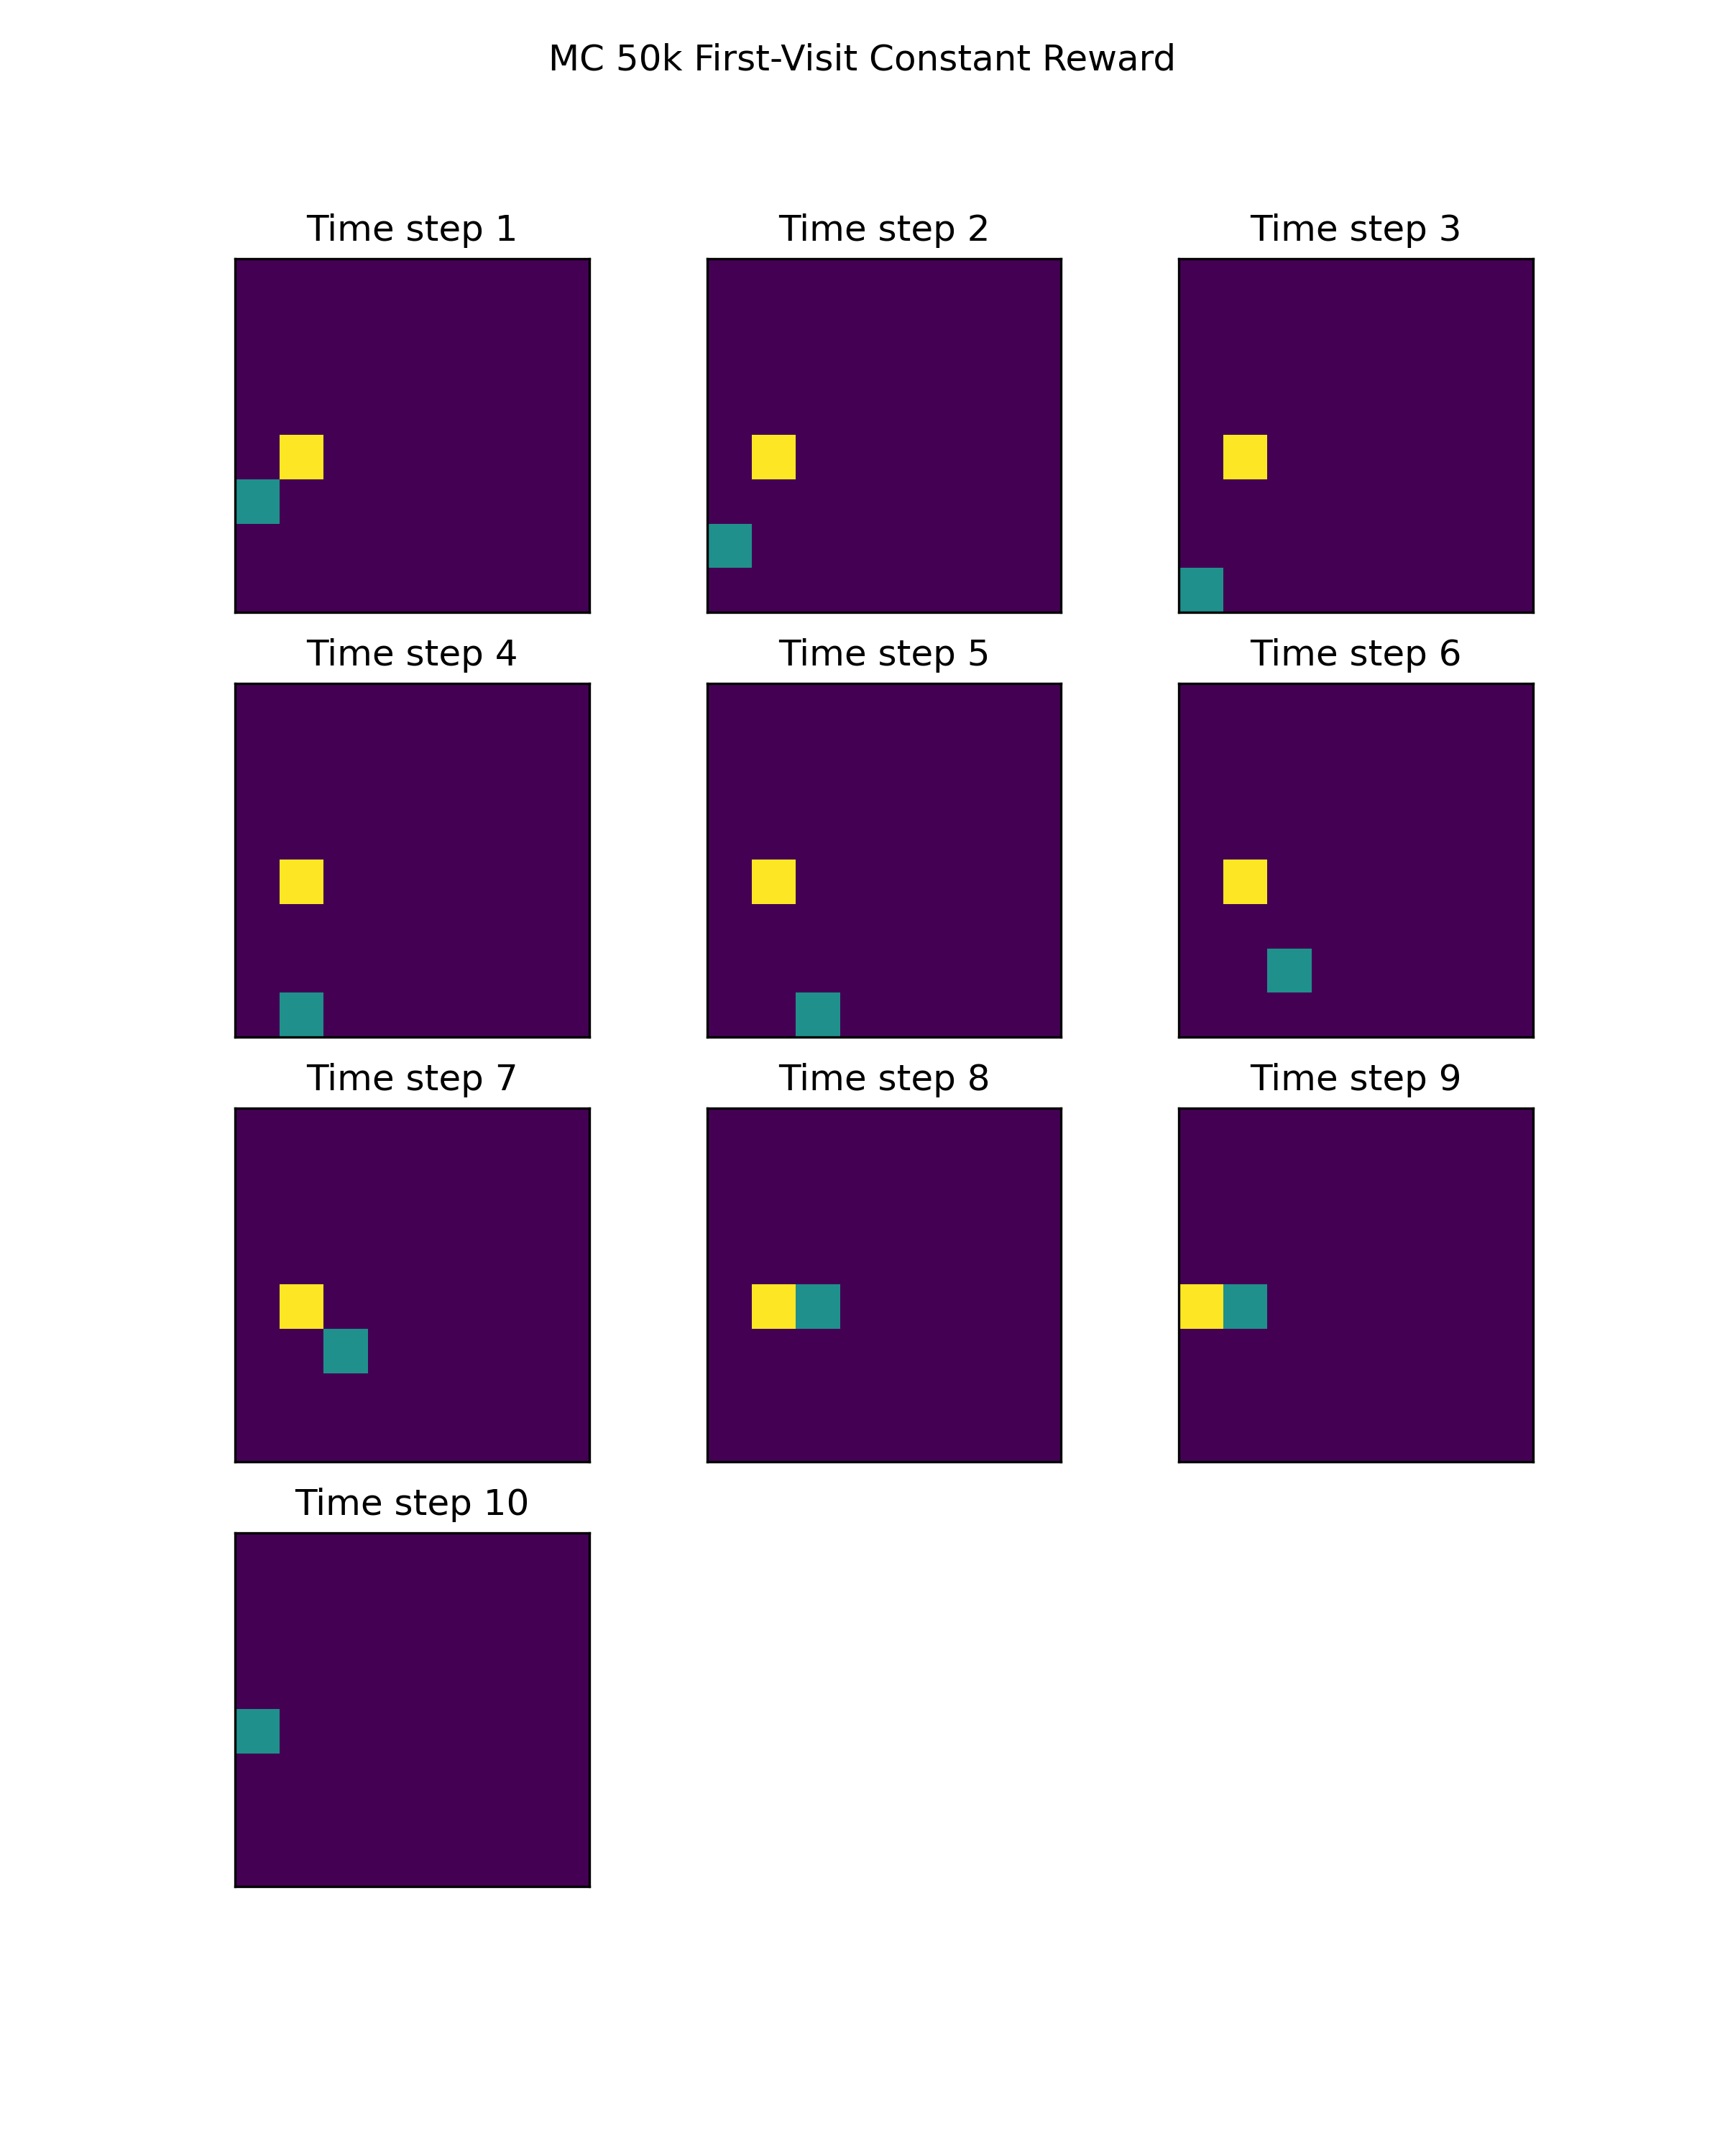
\includegraphics[width=0.95\linewidth]{Figures/mc-50k-first-visit-constant-reward.png}
  \centering
  \label{fig:mcc}
  \caption{The path taken by the First-Visit Monte Carlo robot with a Constant Reward. Blue-green is the robot. Yellow is the bomb.}
\end{figure}

\paragraph{Part c}

\textbf{Q-Learning with a Dynamic Reward and a Uniform Policy}
\begin{itemize}
  \item Q((robotX: 0, robotY: 5), (bombX: 1, bombY: 4)) = [N: 10.00, E: 11.00, S: 9.00, W: 10.00]
  \item Q((robotX: 1, robotY: 5), (bombX: 1, bombY: 4)) = [N: 12.00, E: 10.00, S: 10.00, W: 10.00]
  \item Q((robotX: 1, robotY: 4), (bombX: 1, bombY: 3)) = [N: 13.00, E: 11.00, S: 11.00, W: 11.00]
  \item Q((robotX: 1, robotY: 3), (bombX: 1, bombY: 2)) = [N: 12.00, E: 10.00, S: 10.00, W: 10.00]
  \item Q((robotX: 1, robotY: 2), (bombX: 1, bombY: 1)) = [N: 11.00, E: 9.00, S: 9.00, W: 9.00]
  \item Q((robotX: 1, robotY: 1), (bombX: 1, bombY: 0)) = [N: 10.00, E: 9.00, S: 8.00, W: 8.00]
\end{itemize}

Similar to the constant reward Q's, because the uniform policy causes us to explore constantly, our Q estimates become perfect. In a way, because this has run so long, the forced exploration has essentially solved this problem for all states.

\textbf{Q-Learning with a Dynamic Reward and a Greedy Policy}
\begin{itemize}
  \item Q((robotX: 0, robotY: 5), (bombX: 1, bombY: 4)) = [N: 0.12, E: 4.71, S: -0.20, W: 0.40]
  \item Q((robotX: 1, robotY: 5), (bombX: 1, bombY: 4)) = [N: 4.66, E: 9.00, S: -0.09, W: 0.16]
  \item Q((robotX: 2, robotY: 5), (bombX: 1, bombY: 4)) = [N: 10.00, E: 4.23, S: 4.03, W: 3.22]
  \item Q((robotX: 2, robotY: 4), (bombX: 1, bombY: 4)) = [N: 8.94, E: 8.84, S: 8.95, W: 11.00]
  \item Q((robotX: 1, robotY: 4), (bombX: 0, bombY: 4)) = [N: 7.99, E: 7.94, S: 7.95, W: 10.00]
\end{itemize}

Similar to the greedy policy from before, the Q's are not nearly perfect estimates, however they highest Q's do correspond to the correct actions. While we explore a little bit, we're able to get a ``good-enough'' estimate for Q very quickly. And once we get that ``good-enough'' estimate, we don't explore enough to find better estimates for the other actions. This tends to be okay though because all that matters is that our estimate for the optimal action is the best, which often happens. Do note that we didn't find the optimal path for the dynamic reward though, likely due to not exploring enough.

\textbf{Monte Carlo First-Visit with a Dynamic Reward}
\begin{itemize}
  \item Q((robotX: 0, robotY: 5), (bombX: 1, bombY: 4)) = [N: -127.28, E: 6.10, S: -78.30, W: -81.98]
  \item Q((robotX: 1, robotY: 5), (bombX: 1, bombY: 4)) = [N: 6.82, E: -18.75, S: -29.49, W: -32.04]
  \item Q((robotX: 1, robotY: 4), (bombX: 1, bombY: 3)) = [N: 2.53, E: 7.84, S: 0.09, W: 4.75]
  \item Q((robotX: 2, robotY: 4), (bombX: 1, bombY: 3)) = [N: 9.31, E: 1.47, S: 4.97, W: 7.26]
  \item Q((robotX: 2, robotY: 3), (bombX: 1, bombY: 3)) = [N: 5.91, E: 6.12, S: 7.30, W: 10.61]
  \item Q((robotX: 1, robotY: 3), (bombX: 0, bombY: 3)) = [N: 7.88, E: 7.54, S: 7.51, W: 10.00]
  \item Q((robotX: 2, robotY: 3), (bombX: 0, bombY: 3)) = [N: -34.73, E: -33.75, S: -93.51, W: 8.79]
  \item Q((robotX: 1, robotY: 3), (bombX: 0, bombY: 3)) = [N: 7.88, E: 7.54, S: 7.51, W: 10.00]
\end{itemize}

Similar to the MC learner with the constant reward, our estimates are very far off. Again this can be attributed to the lack of discounting factor, the possibility of staying with the first episode that terminates from that position, and the lack of exploration.


Overall, the reward structure has very little to do with the final Q estimates other than their values (being positive / negative). In all three cases, each method learned roughly the same across the two reward structures.

The path taken by \textbf{Q-Learning with a Dynamic Reward and a Uniform Policy} is shown in Figure \ref{fig:qdu}. It makes sense that we found the optimal path because a our Q estimates have converged perfectly for this scenario and our final policy can easily find the optimal 6-move path for the dynamic reward scenario. The path taken by \textbf{Q-Learning with a Dynamic Reward and a Greedy Policy} is shown in Figure \ref{fig:qdg}. Similar to the uniform policy Q learner, this one has near-perfect Q estimates and can still easily find a near-optimal path, but it is likely not finding the optimal path due to not exploring enough. And the path taken by \textbf{Monte Carlo First-Visit with a Dynamic Reward} is shown in Figure \ref{fig:mcd}. The Monte Carlo path closer to a near optimal path this time. Again, the reason for this is partially due to a lack of exploration and partially due to the chances of finding a short episode (and therefore smaller Q values) is very unlikely.

Overall, forcing the learners to explore, while slow, does seem to produce optimal solutions.

\begin{figure}
  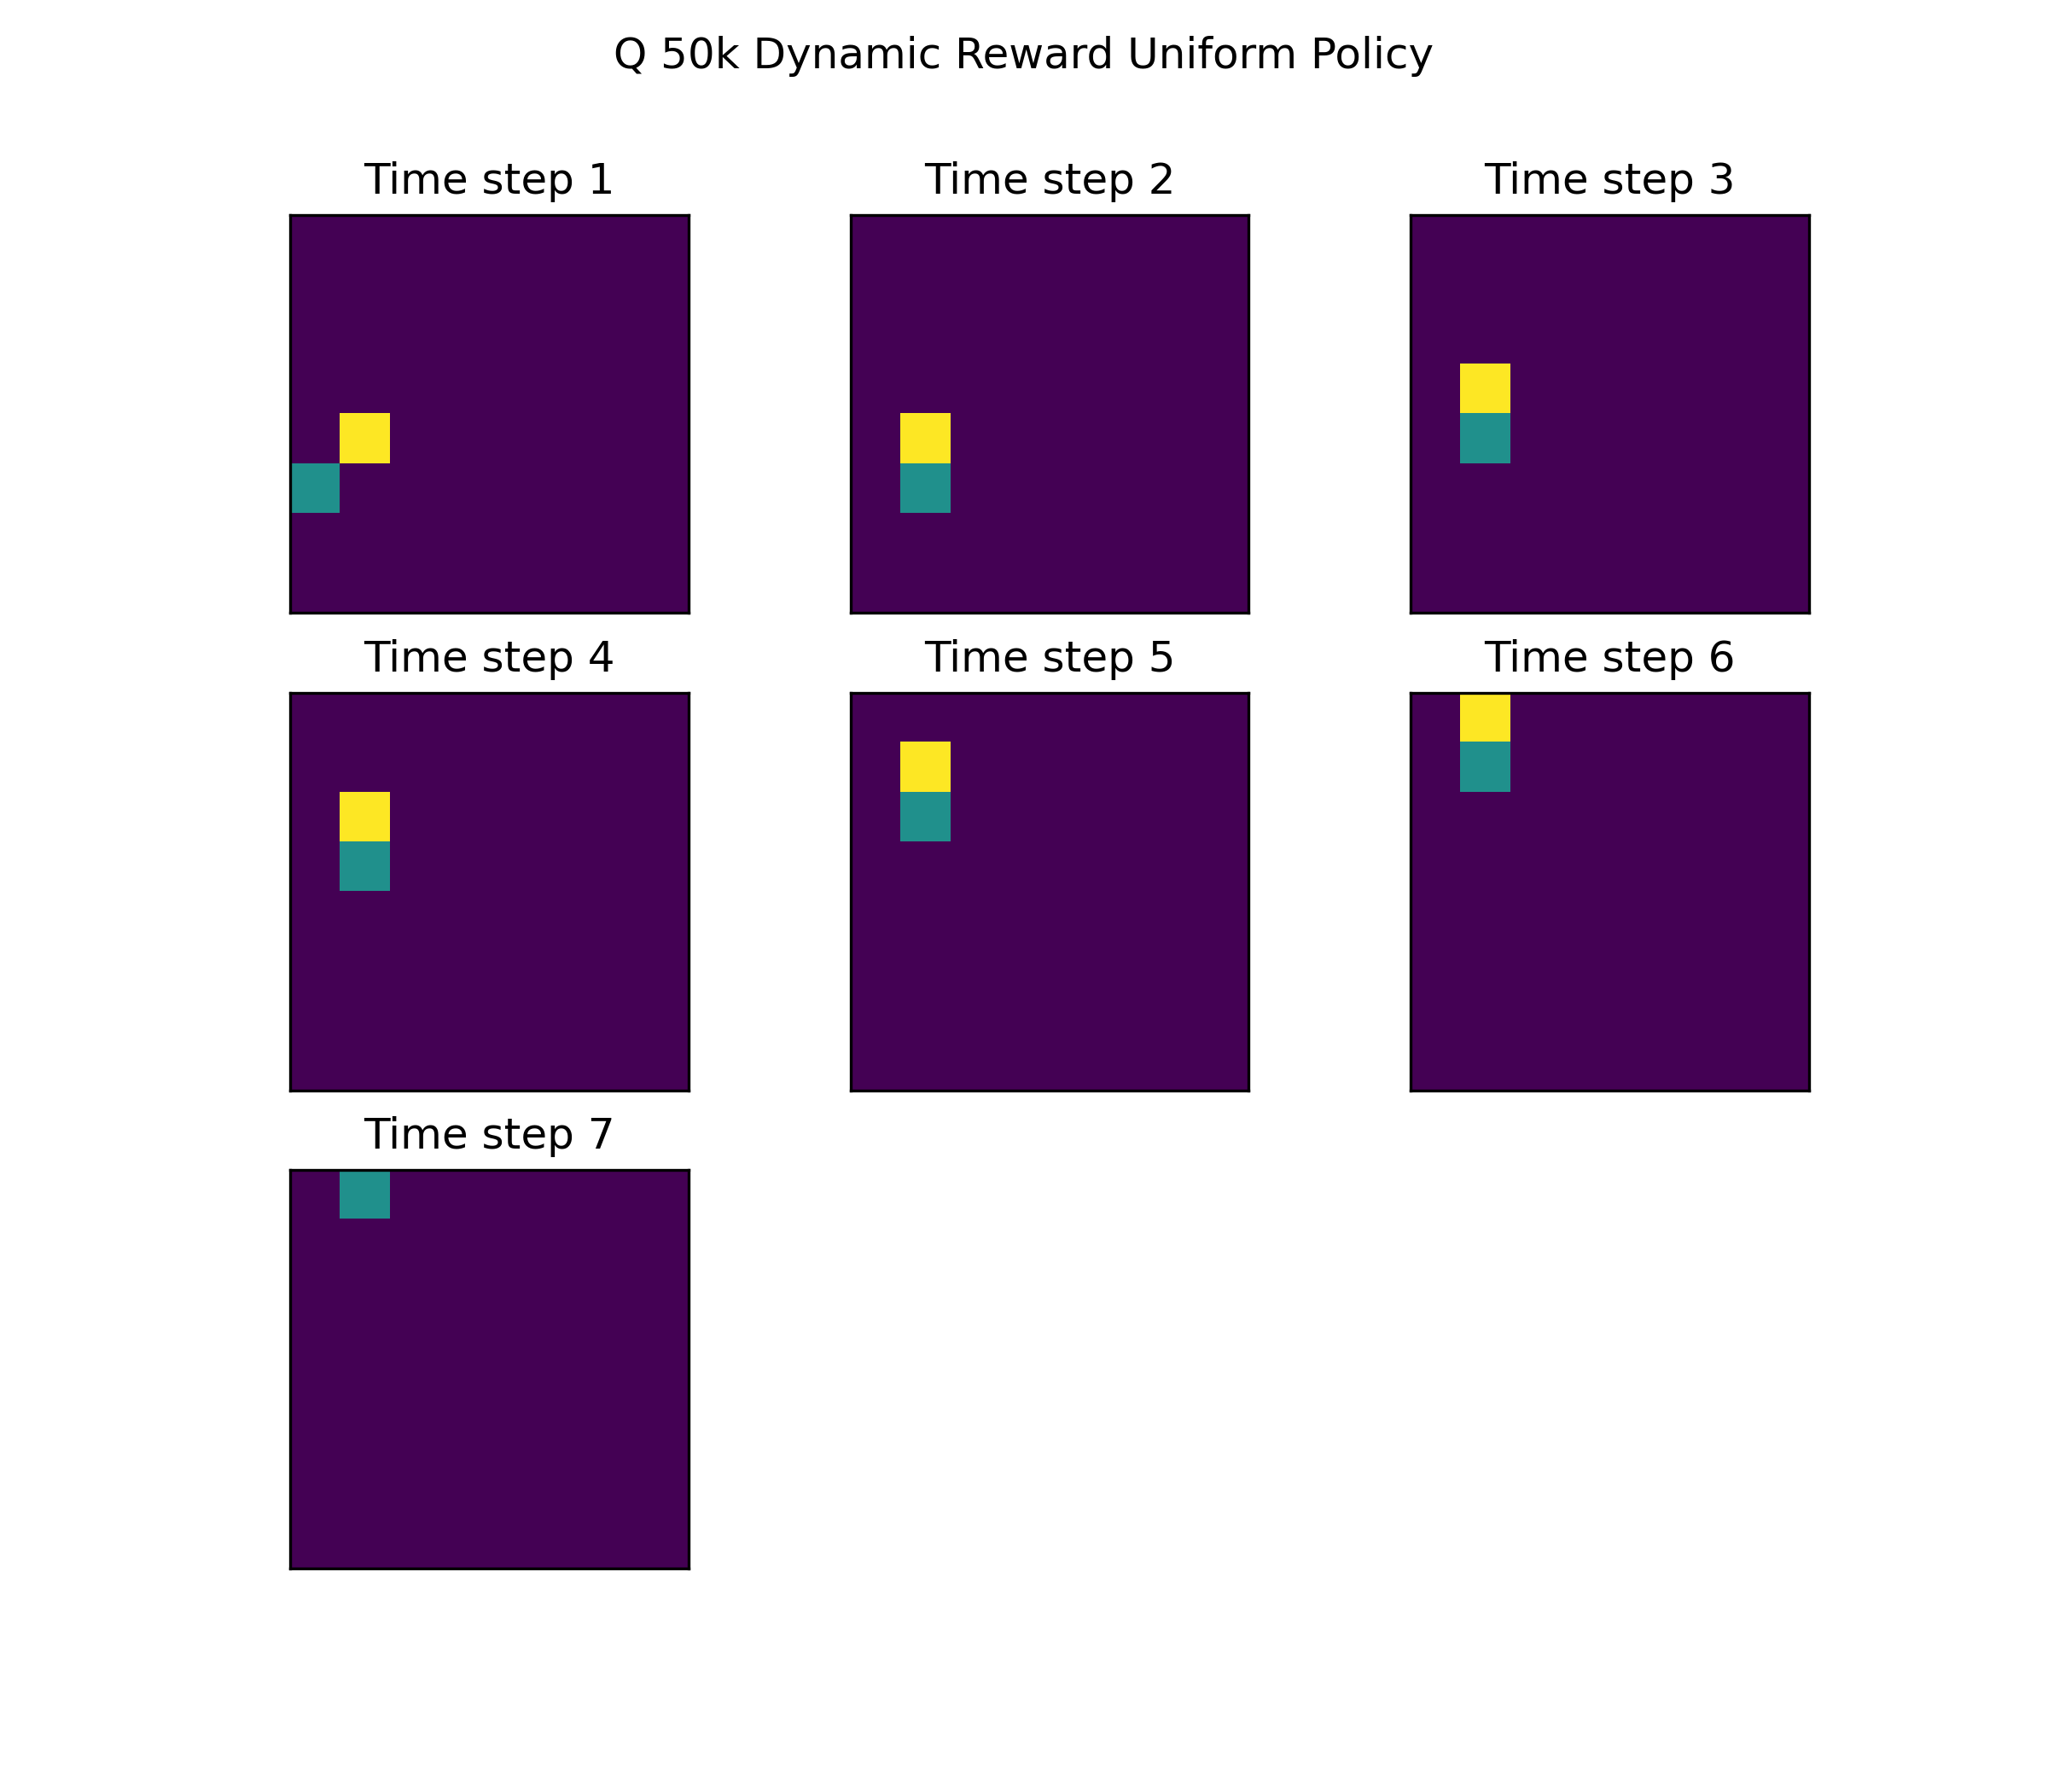
\includegraphics[width=0.95\linewidth]{Figures/q-50k-dynamic-reward-uniform-policy.png}
  \centering
  \caption{The path taken by the Q-Learning robot with a Dynamic Reward and a Uniform Policy. Blue-green is the robot. Yellow is the bomb.}
  \label{fig:qdu}
\end{figure}

\begin{figure}
  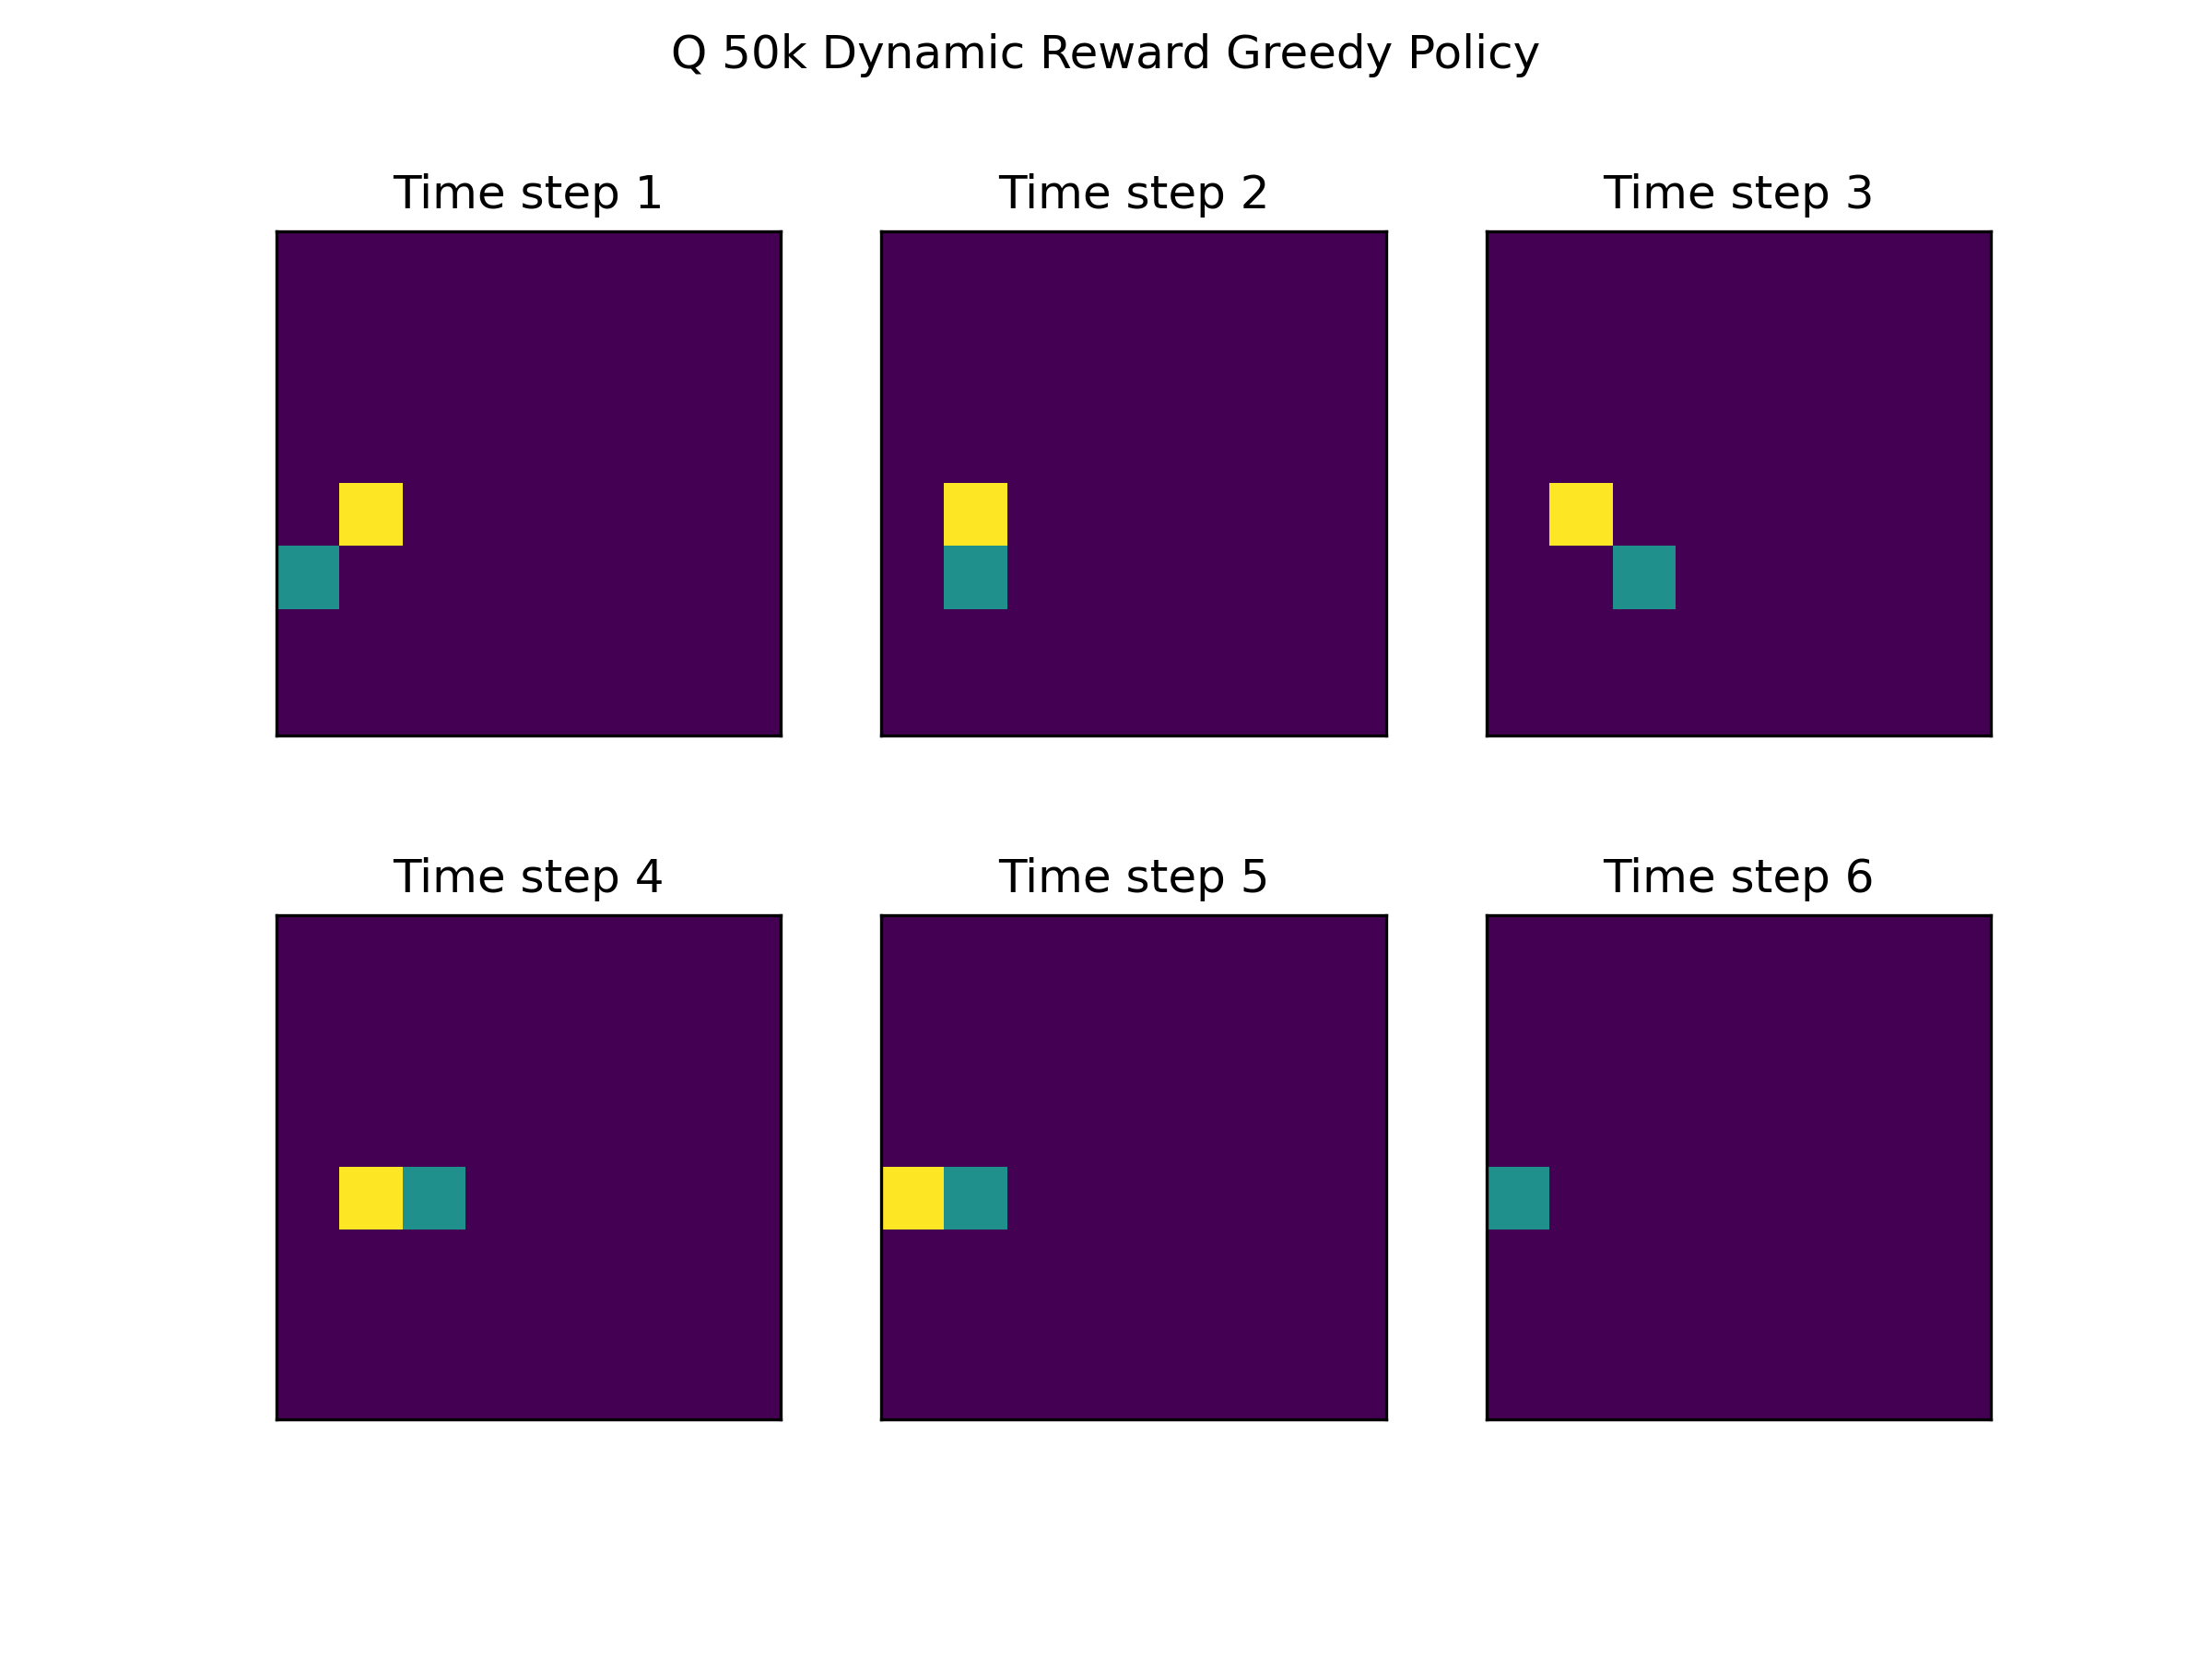
\includegraphics[width=0.95\linewidth]{Figures/q-50k-dynamic-reward-greedy-policy.png}
  \centering
  \caption{The path taken by the Q-Learning robot with a Dynamic Reward and a Greedy Policy. Blue-green is the robot. Yellow is the bomb.}
  \label{fig:qdg}
\end{figure}

\begin{figure}
  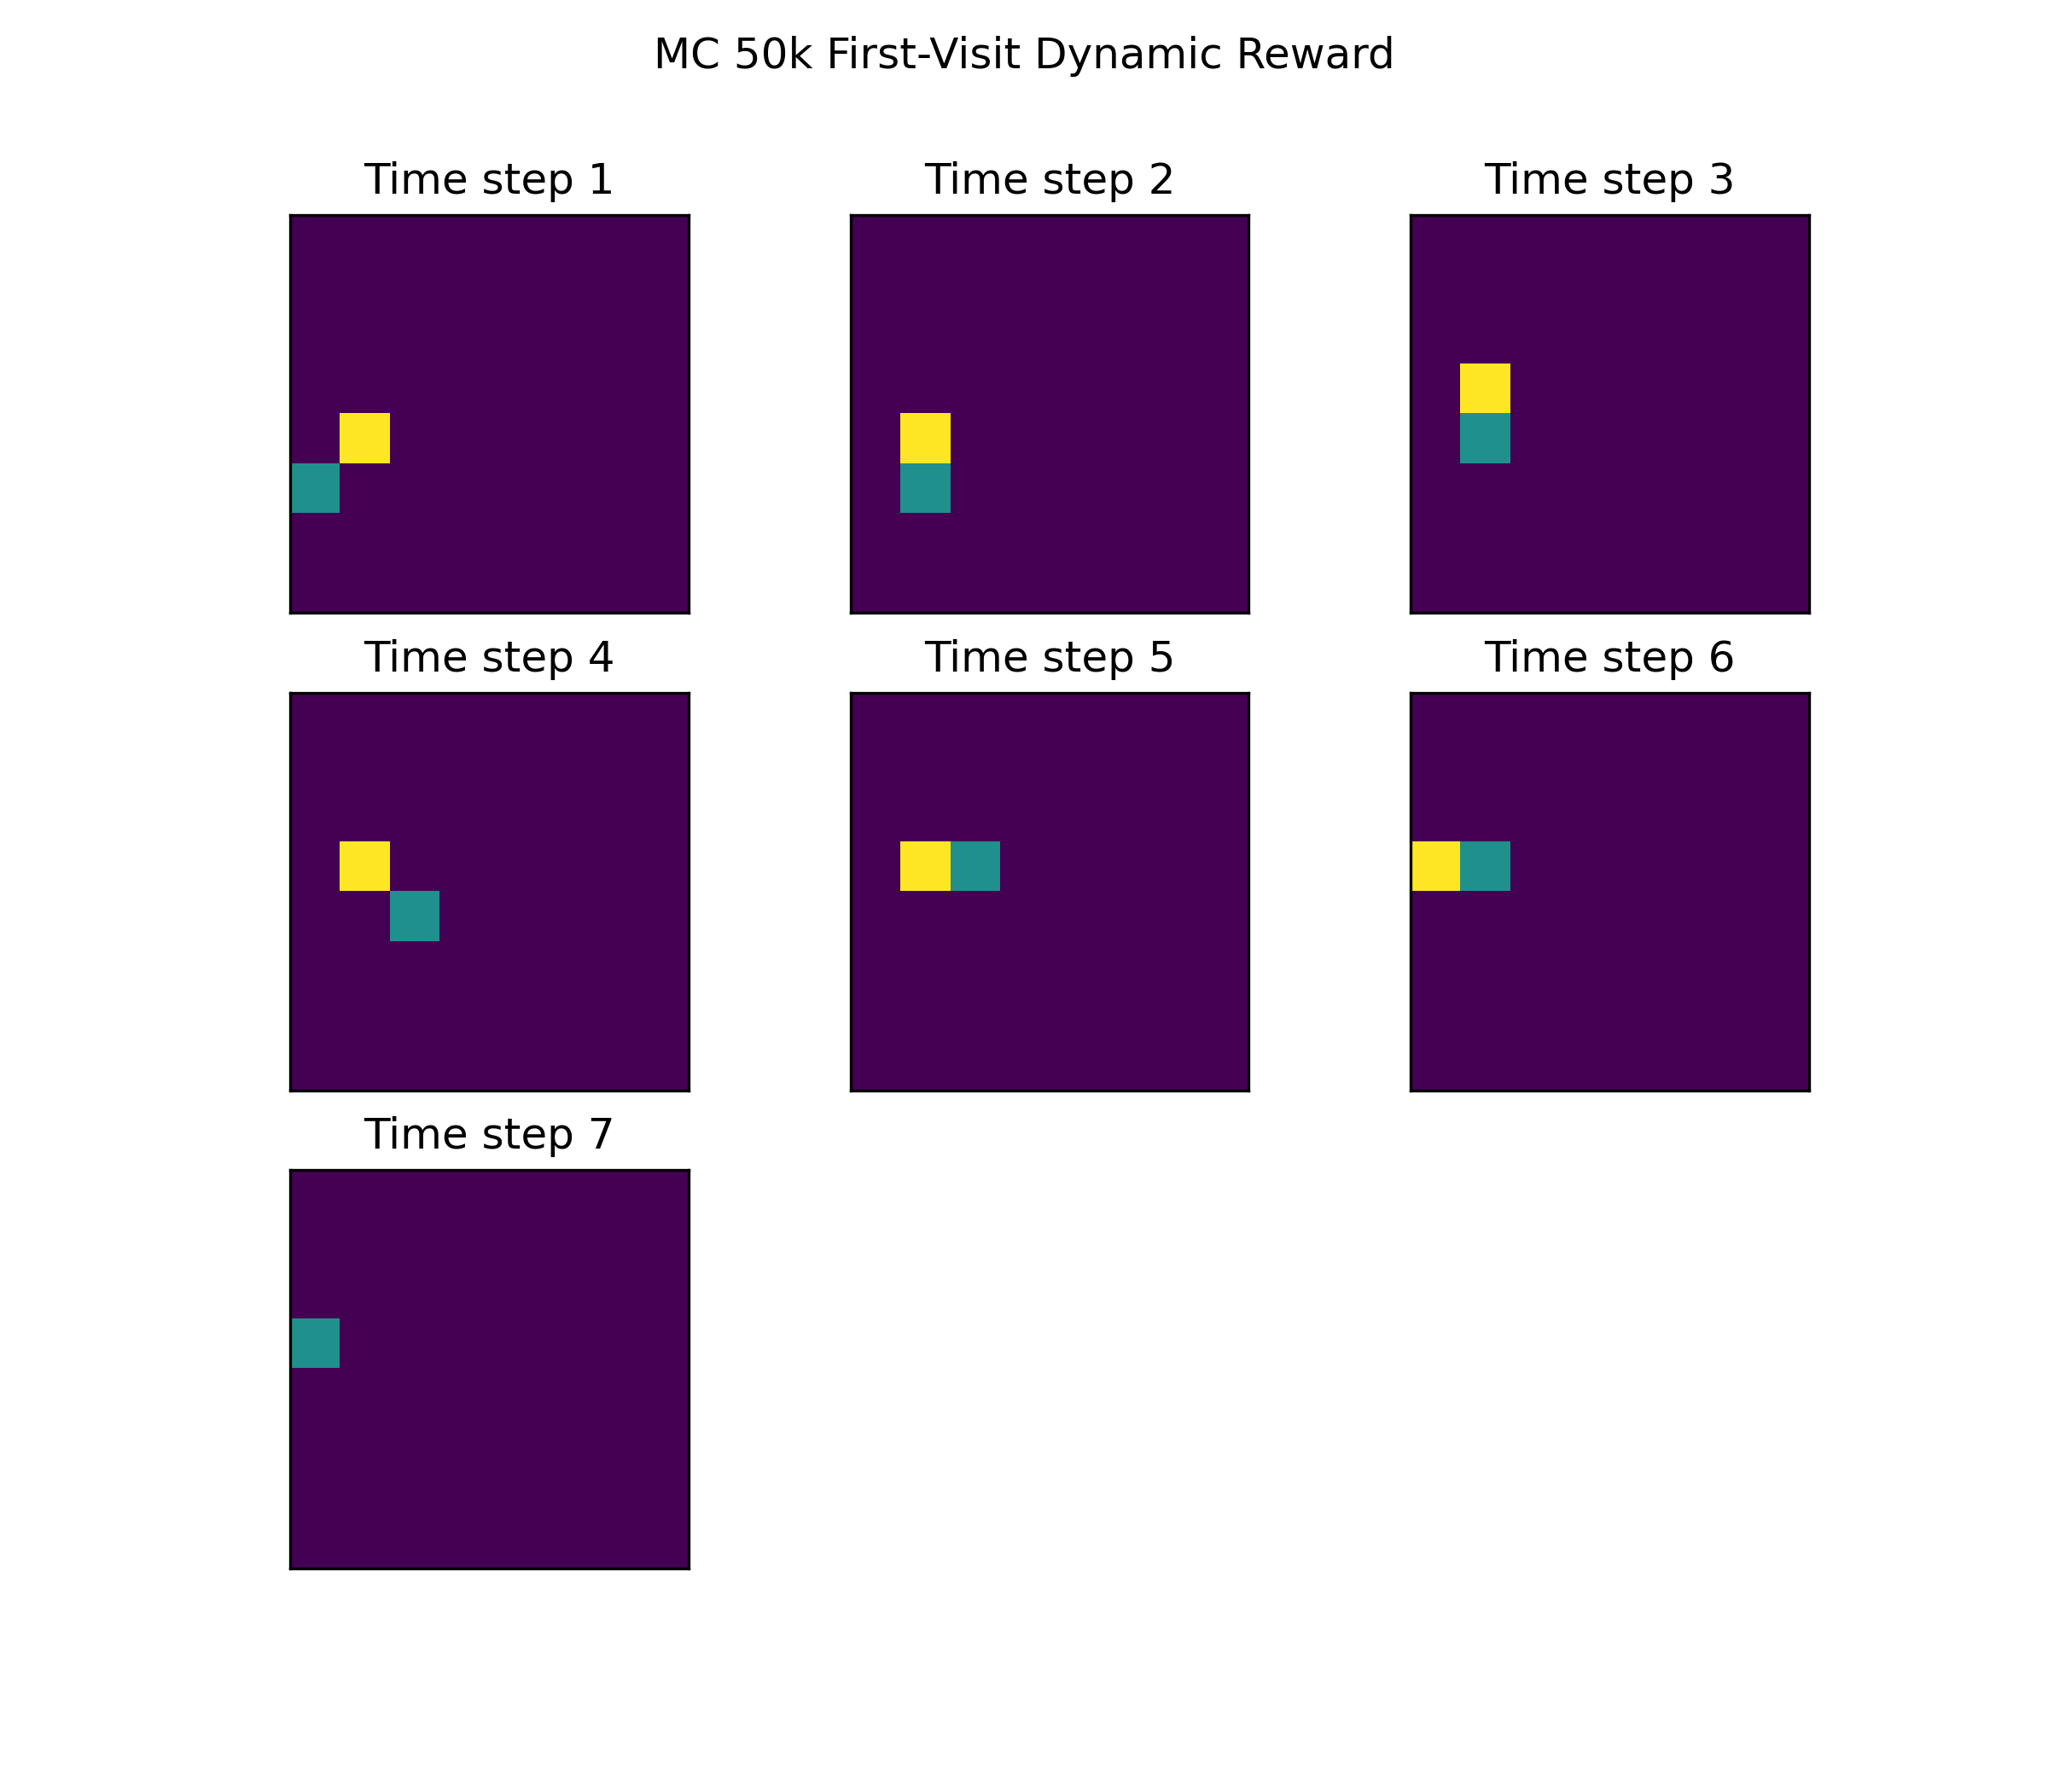
\includegraphics[width=0.95\linewidth]{Figures/mc-50k-first-visit-dynamic-reward.png}
  \centering
  \caption{The path taken by the First-Visit Monte Carlo robot with a Dynamic Reward. Blue-green is the robot. Yellow is the bomb.}
  \label{fig:mcd}
\end{figure}

\paragraph{Part d}

Because we went through 50k episodes, the graphs for rewards per episode is messy. A better graph would be the average reward over runs.

In Figure \ref{fig:crvt}, I show the reward per episode using a constant reward structure for all three methods: MC Learning, Q-Learning with a Greedy Policy, and Q-Learning with a Uniform Policy. As we can see, it's fairly messy to understand. I've devised a slightly different graph to better show the reward per episode that I deem the average reward per run which is a rolling average calculated like so, where i is the episode number:
$$
  Avg(i) = \frac{\sum_1^i R_i}{i}
$$

In Figure \ref{fig:crt}, I show the average reward per episode using a constant reward structure. From these two graphs, we can see that the episodes generated Q-Learning with a Greedy Policy have a very high reward. Monte Carlo achieves similar results, but it takes a lot more episodes to get there. It's harder to determine the learning of Q-Learning with a Uniform Policy because the episodes it generates are always random.

\begin{figure}
  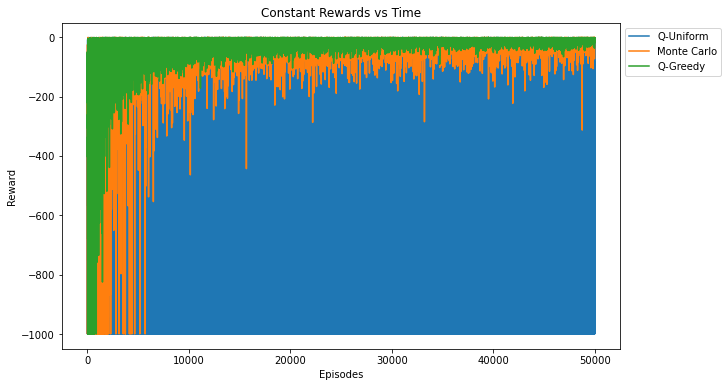
\includegraphics[width=0.95\linewidth]{Figures/constant-rewards-vs-time.png}
  \centering
  \caption{Rewards per episode using a constant reward structure.}
  \label{fig:crvt}
\end{figure}

\begin{figure}
  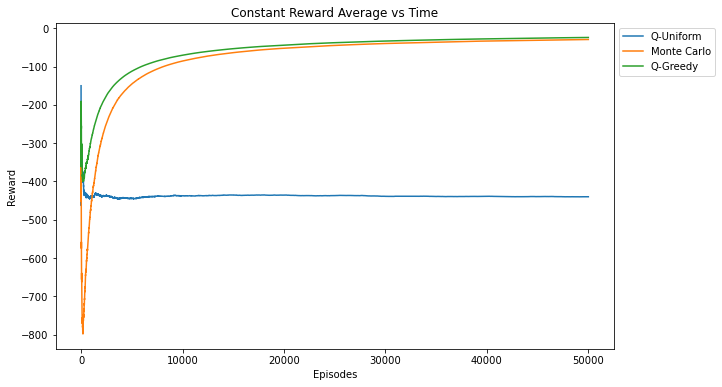
\includegraphics[width=0.95\linewidth]{Figures/constant-reward-average-vs-time.png}
  \centering
  \caption{Average reward per episode using a constant reward structure.}
  \label{fig:crt}
\end{figure}

In Figure \ref{fig:drvt}, I show the reward per episode using a dynamic reward structure for all three methods: MC Learning, Q-Learning with a Greedy Policy, and Q-Learning with a Uniform Policy. Similar to the constant reward structure results, it's also messy to understand. So in Figure \ref{fig:drt}, I show the average reward per episode using a dynamic reward structure. From these two graphs, we can see that the episodes generated Q-Learning with a Greedy Policy have a very high reward and learn very very fast compared to when using a constant reward structure. Monte Carlo achieves similar results when using either reward structure. And again it's still harder to determine the learning of Q-Learning with a Uniform Policy because the episodes it generates are always random.

Both of these sets of results make sense because regardless of reward structure, Monte Carlo takes a good amount of successful episodes to learn something useful and that's why the results for Monte Carlo are roughly the same across both. For Q-Learning, the dynamic reward structure gives us better estimates short term for the cases where we move the bomb further away from the center and prevent Q values from exploding when we have an unsuccessful episode.


\begin{figure}
  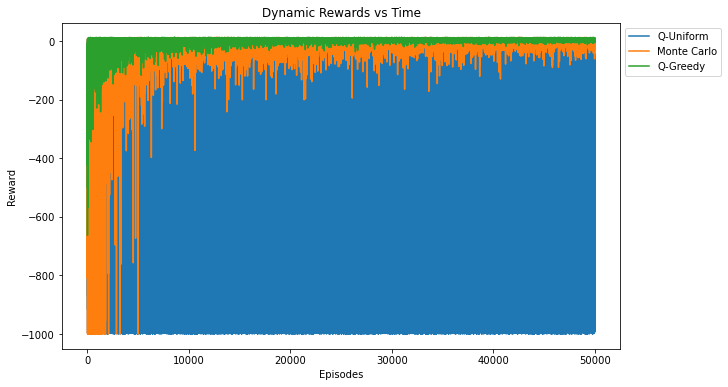
\includegraphics[width=0.95\linewidth]{Figures/dynamic-rewards-vs-time.png}
  \centering
  \caption{Rewards per episode using a dynamic reward structure.}
  \label{fig:drvt}
\end{figure}

\begin{figure}
  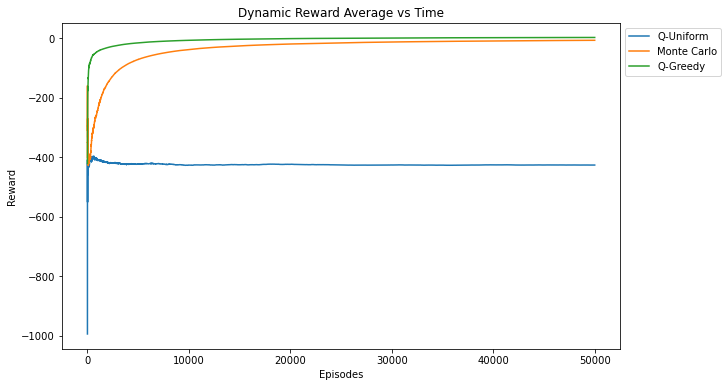
\includegraphics[width=0.95\linewidth]{Figures/dynamic-reward-average-vs-time.png}
  \centering
  \caption{Average reward per episode using a dynamic reward structure.}
  \label{fig:drt}
\end{figure}

\paragraph{Part e}

In Figure \ref{fig:crts} I show the time taken up to each episode versus the number of episodes ran using a constant reward. In Figure \ref{fig:drts} I show the same graph but for dynamic rewards. In both cases, the Q-Learner with the uniform policy takes the longest --- this makes sense because each episode is essentially random, we aren't using any learned knowledge to dictate our episodes so learning takes a long time. In the case of Monte Carlo and Q-Learning with the greedy policy start to go a lot faster once they learn a near-optimal policy because they're using their learned knowledge to generate episodes.

\begin{figure}
  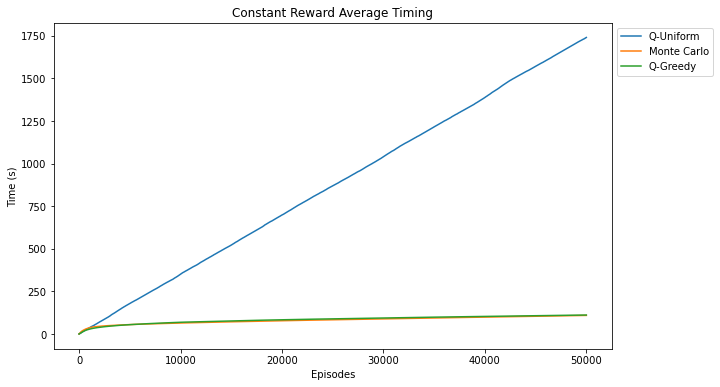
\includegraphics[width=0.95\linewidth]{Figures/constant-reward-timing.png}
  \centering
  \caption{Total time taken for each learning method vs episodes using a constant reward structure.}
  \label{fig:crts}
\end{figure}

\begin{figure}
  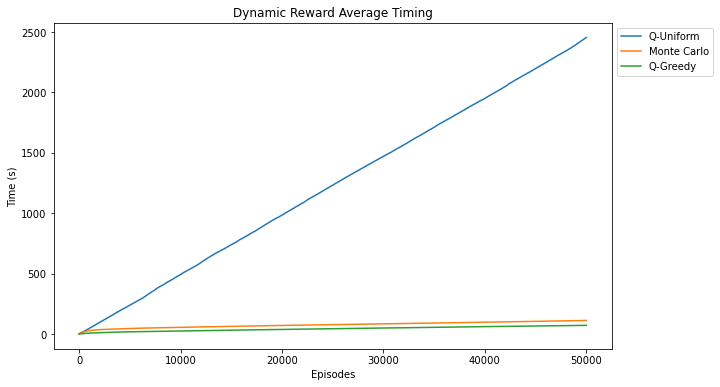
\includegraphics[width=0.95\linewidth]{Figures/dynamic-reward-timing.png}
  \centering
  \caption{Total time taken for each learning method vs episodes using a dynamic reward structure.}
  \label{fig:drts}
\end{figure}

\section{Conclusion}

Overall we've tested 3 different learning methods using 2 different reward structures to see how well they perform in both finding the optimal solutions to the robot-bomb problem and how long they take to train. From these results we can conclude that MC learning, while able to find a near-optimal policy, performs worse than both Q-learners in performance, and only better than Q-Uniform in terms of time taken. And between the two Q-learners, the one with the uniform policy ends up with the better final policy than the one using the greedy policy, but it takes much longer to train. The main take away is that each method has its pros and cons and are all viable candidates at solving basic Reinforcement Learning problems.

\bibliographystyle{abbrv}
\bibliography{main}

\end{document}